\section{Background due to Natural Radioactivity in the Detector and Shield Components}
\label{secDetectorMaterials}

Decays of the radioactive isotopes in the materials listed in Table~\ref{tabScreeningResults} have been simulated with GEANT4 using the detailed detector model (see Section~\ref{secGeant4model}), and the corresponding expected background rates have been calculated. The measured radioactive contamination (Section~\ref{secScreening}) has been used as an input information for the background predictions. For the analysis presented here, the upper limits are treated as detection values.

Figure~\ref{figSpectraFS_1} shows the spectra in the entire energy range, and Figure~\ref{figSpectraFS_2} in the low energy region of interest. The latter has been chosen to be sufficiently wide, up to 100~keV, to include the signal region for inelastic dark matter which is predicted to be in a higher energy range than the one from standard elastic WIMP scattering~\cite{inelasticDM1, inelasticDM2}.  The effect of the discrimination between multiple and single scatter events can be seen in Figure~\ref{figSpectraFS}: the multiple scatter behavior of incident gamma rays is typical for higher energies, whereas single scatter events dominate in the low energy region and the multiple scatter cut does not yield a significant reduction of the background rate. Further background reduction can be achieved with fiducial volume cuts, where the outer part of the  target volume is not considered for analysis, exploiting the self-shielding capabilities of liquid xenon.

\begin{figure}[!h]
\centering
\subfigure[]{
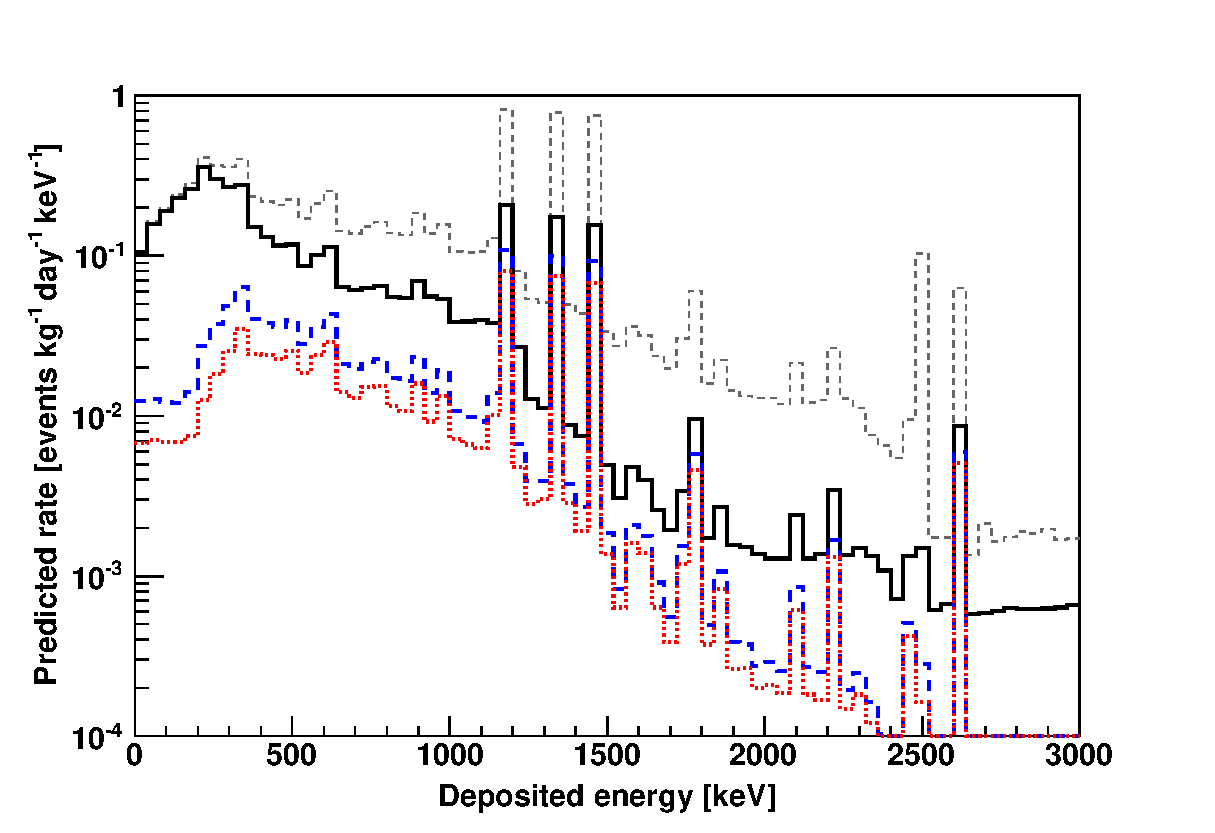
\includegraphics[width=0.475\linewidth]{plots/BackgroundMaterials/SpectraFS_withFV40andFV30_75bins_dot.eps}
\label{figSpectraFS_1}}
\subfigure[]{
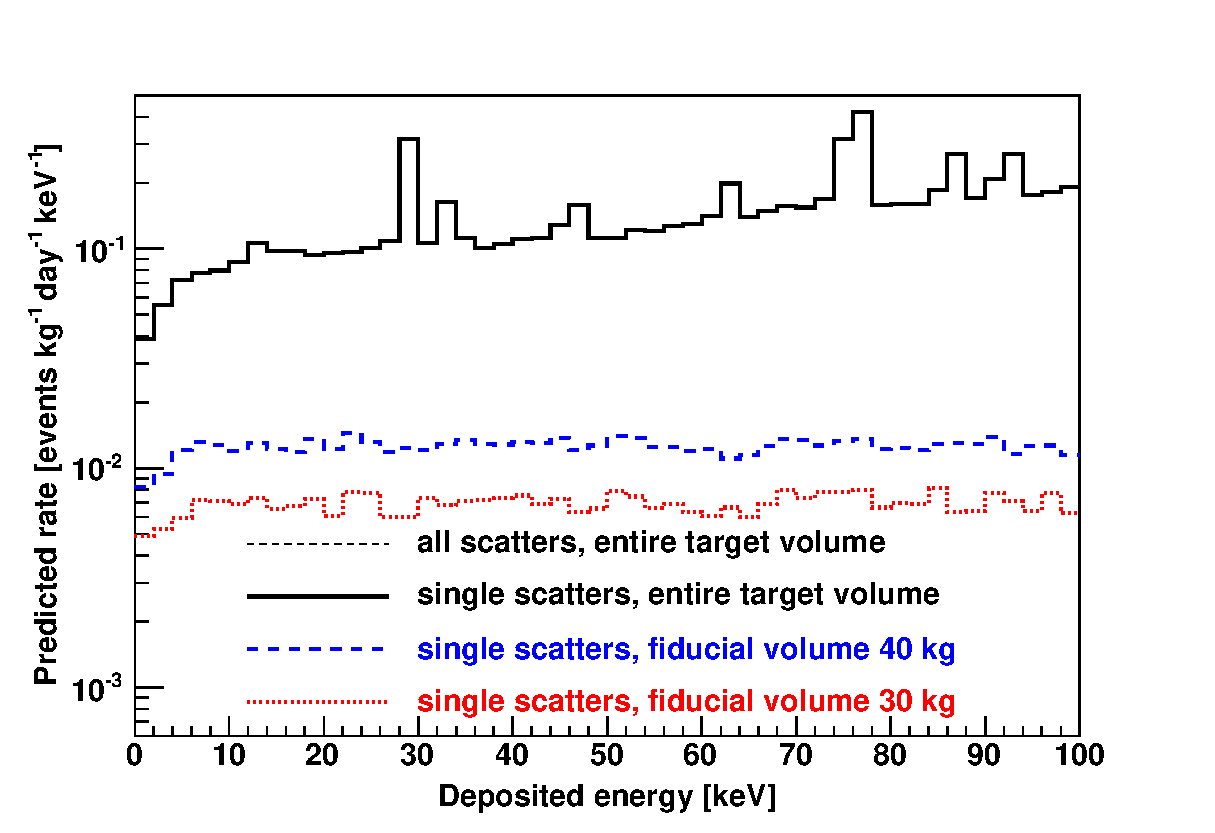
\includegraphics[width=0.475\linewidth]{plots/BackgroundMaterials/SpectraWS_withFV40andFV30_50bins_dot.eps}
\label{figSpectraFS_2}}
\caption[Energy spectra of the predicted background]{Predicted background from the detector and shield materials: (a) - energy spectra of all events (thin dashed line) and single scatters (solid line) in the entire 62~kg LXe target, and single scatters in the 40~kg (thick dashed line) and 30~kg fiducial volumes (dotted line), with infinite energy resolution. (b) - zoom into the low energy region of the Monte Carlo spectra. The spectra of all scatters and single scatter events in the entire target volume overlap. Figures published in Ref.~\cite{EMBG}.}
\label{figSpectraFS}
\end{figure}

In Figure~\ref{figSpectraFS_2}, several characteristic X-rays can be seen. The xenon K-shell fluorescence peaks appear at 30~keV and 34~keV. The X-ray peaks at 15, 75, 85 and 90~keV are from Pb and Bi contamination close to the target volume, for example in the PTFE walls of the TPC. In addition, there is a 46~keV gamma line from the $^{210}$Pb decay, and a 63~keV gamma line from the decay of $^{234}$Th. Due to their short mean free path, these low energy lines can be observed only at the edge of the LXe volume. After applying a fiducial volume cut, the peaks disappear and the spectrum becomes relatively flat in the low energy region. The background rate is thus presented as the average below 100~keV.

\begin{floatingfigure}[lh]{0.475\textwidth}
%\begin{figure}[!h]
\centering
%\begin{tabular}{cc}
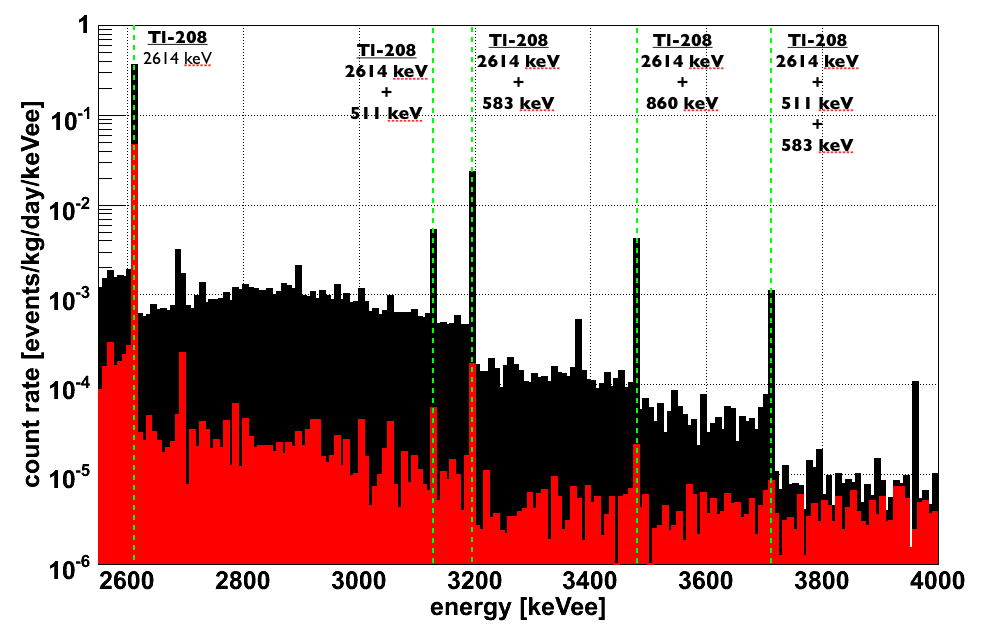
\includegraphics[width=0.475\linewidth]{plots/BackgroundMaterials/Tl208decay.png}
%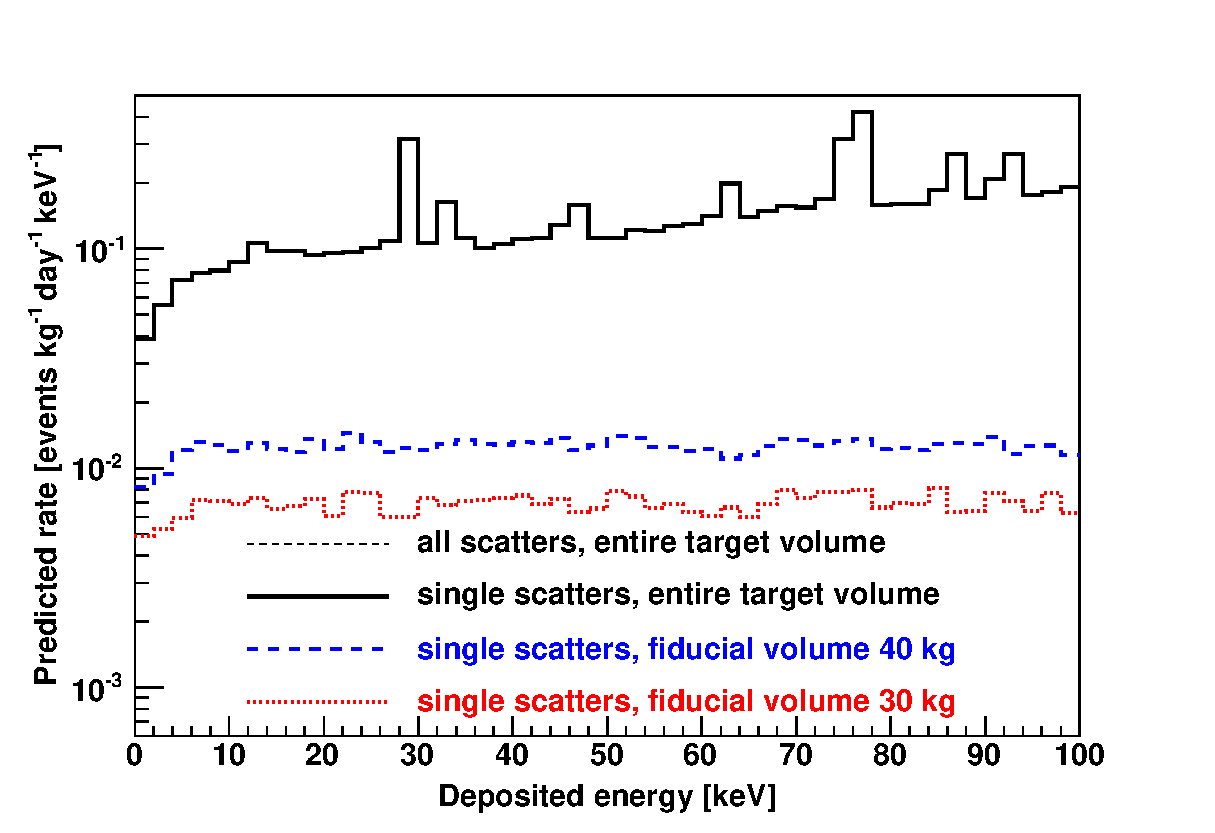
\includegraphics[width=0.5\linewidth]{plots/BackgroundMaterials/SpectraWS_withFV40andFV30_50bins_dot.eps}
%\end{tabular}
\caption[High energy part of the simulated background spectrum, pile-up peaks from $^{208}$Tl decay]{High energy part of the simulated background spectrum, pile-up $\gamma$-lines from $^{208}$Tl decay. Black histogram - all events, red - single scatter interactions.}
\label{figTl208}
%\end{figure}
\end{floatingfigure}

The events with energies above 2.6~MeV seen in Fig.~\ref{figSpectraFS_1} are originating mostly from the decay of $^{208}$Tl in the $^{232}$Th decay chain, which undergoes $\beta^{-}$-decay with a Q-value of 5~MeV. Even though the energy of a single emitted photon from the de-excitation of the daughter nucleus $^{208}$Pb does not exceed 2.614~MeV, in some cases it is excited to a higher energy level, and 2 or 3 photons with different energies are emitted almost simultaneously, with a delay time in the order of picoseconds. Due to the finite time and position resolutions of the XENON100 detector (see Section~\ref{secPositionResolution}) they cannot be resolved independently and result in pile-up peaks shown in Fig.~\ref{figTl208}.

The spatial distribution of the single scatter electronic recoil events in the region of interest is presented in Figure~\ref{figPositionDistribution}. The radial cut rejects events at the edge of the target volume, originating mostly from radioactive decays in the PTFE of the TPC and the 316Ti SS of the cryostat vessels.
The background from the PMTs, PMT bases, the diving bell, and the electrodes can be efficiently reduced by rejecting events within the top and bottom layers of LXe.

\begin{figure}[!b]
\subfigure[without veto cut]{
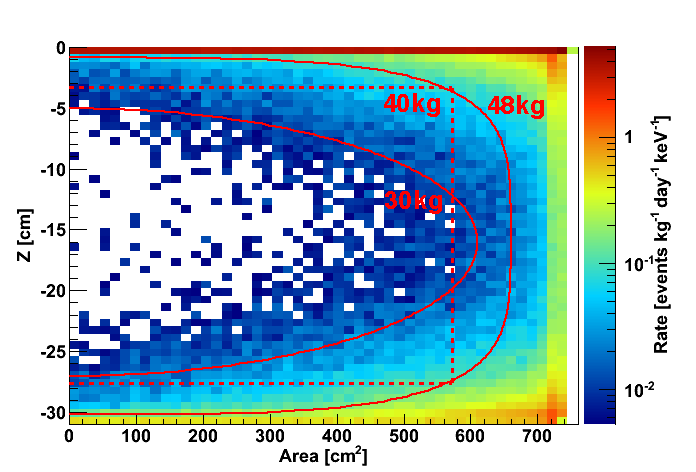
\includegraphics[width=0.475\linewidth]{plots/BackgroundMaterials/AZcolor_ER_PassiveVeto_withLabels1.png}
\label{figPositionDistribution_1}}
\subfigure[with veto coincidence cut]{
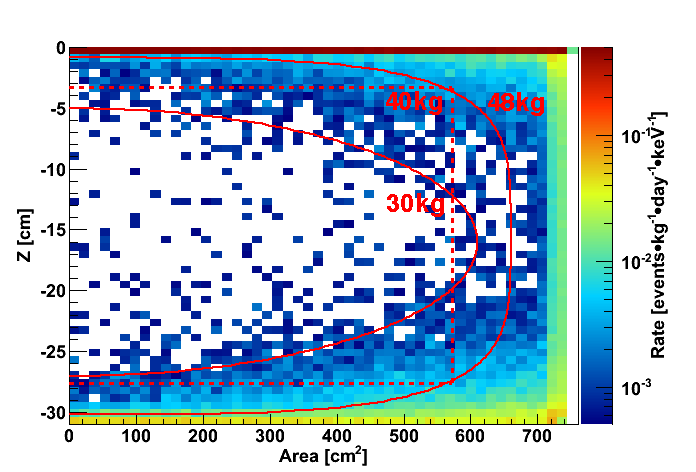
\includegraphics[width=0.475\linewidth]{plots/BackgroundMaterials/AZcolor_ER_ActiveVeto100keV_withLabels1.png}
\label{figPositionDistribution_2}}
\caption[Spatial distribution of the simulated electronic recoil background from detector and shield materials]{Spatial distribution of the simulated electronic recoil background from detector and shield materials, excluding intrinsic radioactivity in the LXe. Shown are single scatter events with energy below 100~keV in the TPC, without veto cut (a) and with a veto coincidence cut (b). $Z$ = 0~cm corresponds to the liquid-gas interface. The cathode mesh is located at $Z$ = $-$304.5~mm. The dashed line shows the 40~kg fiducial volume, and the solid lines illustrate the 48~kg and 30~kg fiducial volumes optimized to minimize the background.}
\label{figPositionDistribution}
\end{figure}

The background has been predicted for the entire 62~kg LXe target, and for three fiducial volumes: a simple 40~kg cylindrical fiducial volume used in the analysis of the XENON100 data from the commissioning run in Fall 2009, on which the first dark matter search results has been obtained~\cite{xe100-run07}, and for the 48~kg and 30~kg fiducial volume cuts designed following the spatial distribution of events in the target volume. The 48~kg fiducial volume has been used in the analysis of the first scientific run~\cite{xe100-run08}, and the 30~kg cut is optimized to minimize the extrinsic background for the spectroscopy analysis of the measured background spectrum described in Section~\ref{secDataMCcomparison}. 

%\begin{floatingfigure}[r]{0.475\textwidth}
\begin{figure}[!t]
\subfigure[]{
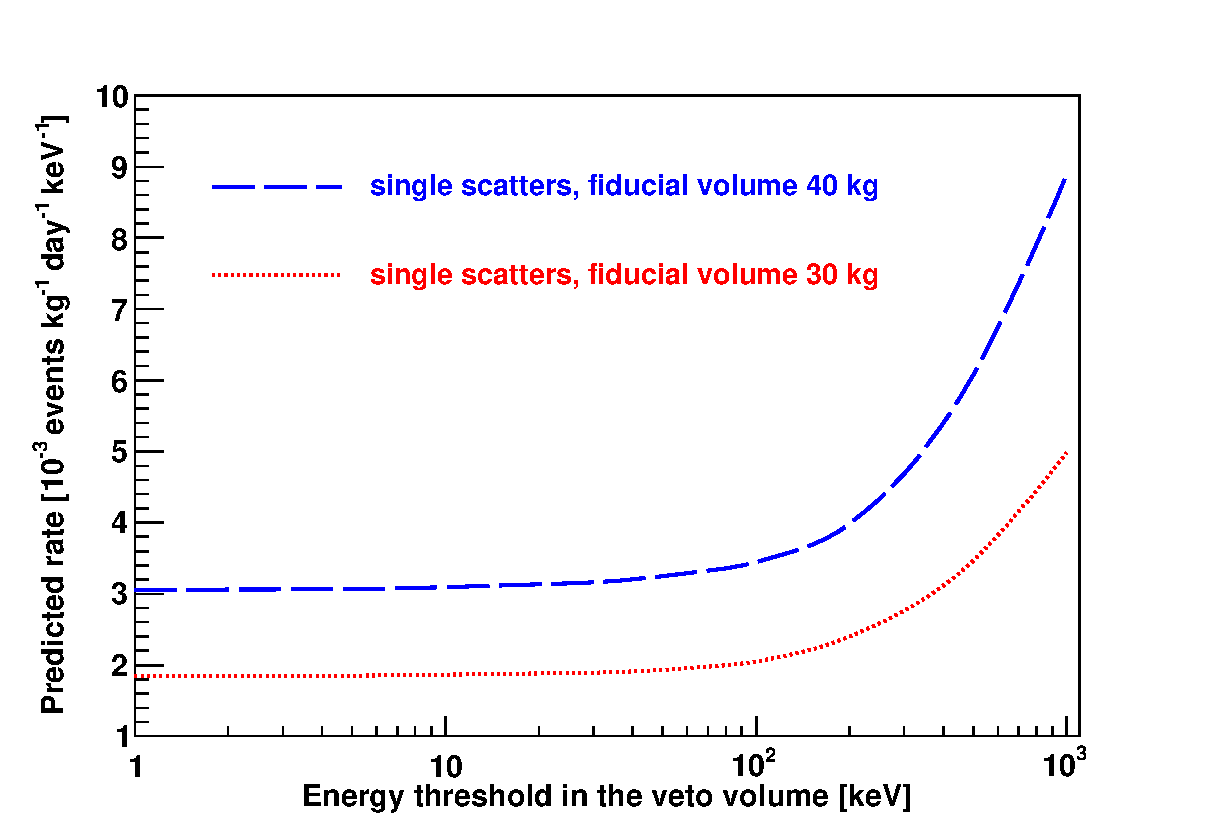
\includegraphics[width=0.475\linewidth]{plots/BackgroundMaterials/VetoReduction_linear_dot.eps}
\label{figVetoCuts_1}}
\subfigure[]{
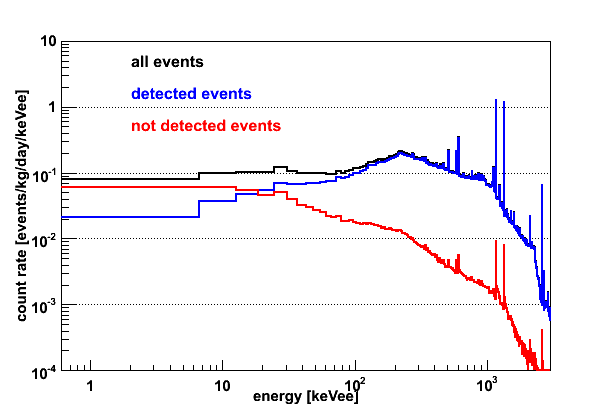
\includegraphics[width=0.475\linewidth]{plots/VetoMeasurement/etotv_all.png}
\label{figVetoCuts_2}}
\caption[Predicted background rate from the detector and shield materials in the energy range below 100~keV, as a function of the energy threshold in the active veto]{(a) - predicted background rate from the detector and shield materials in the energy range below 100~keV, as a function of the energy threshold in the active veto. The average energy threshold in the veto measured with a collimated $^{137}$Cs source is about 100~keV. Figure published in Ref.~\cite{EMBG}. (b) - energy deposited in the veto volume from a Monte Carlo simulation with an infinite energy resolution. The events which are not below the energy threshold in the veto contribute to the background in the target volume.}
\label{figVetoCuts}
\end{figure}
%\end{floatingfigure}

%\begin{floatingfigure}[r]{0.5\textwidth}
\begin{figure}[!b]
\centering
\subfigure[]{
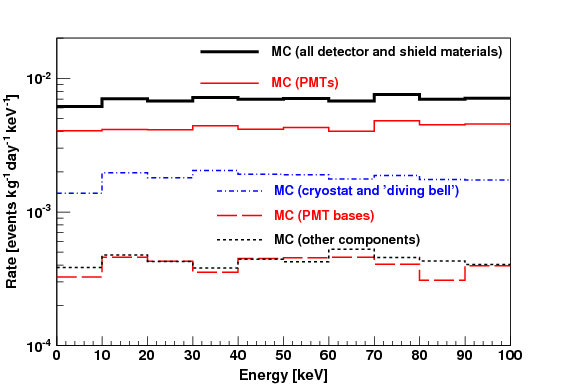
\includegraphics[width=0.475\linewidth]{plots/BackgroundMaterials/DetectorMaterials_FV30superellipse_PassiveVeto.png}
\label{figSpectraDetectorMaterials_1}}
\subfigure[]{
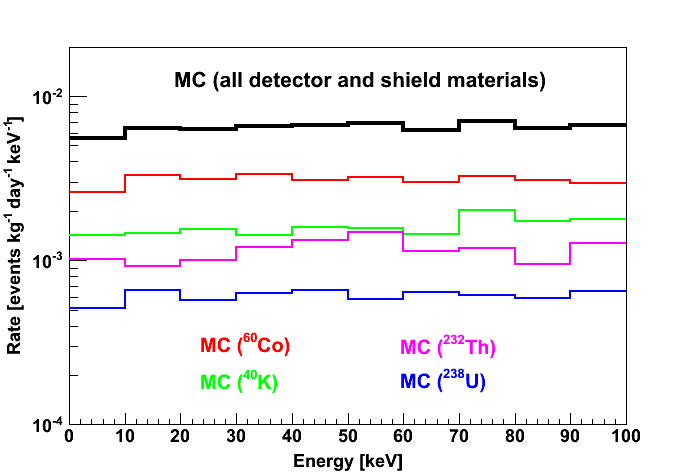
\includegraphics[width=0.475\linewidth]{plots/BackgroundMaterials/ChainsContributions.png}
\label{figSpectraDetectorMaterials_2}}
\caption[Contribution to the background from different components and decay chains]{(a) - predicted background from the detector and shield components (thick black line) in 30~kg fiducial mass without veto cut, together with the individual contributions from the PMTs (solid line), the cryostat with pipes and diving bell (dash dotted line), and PMT bases (long dashed line). The short dashed line shows the summed background from all other components: detector PTFE and copper, cryostat support bars, TPC resistor chain, top and bottom electrodes, PMT cables, and copper and polyethylene shield. Figure published in Ref.~\cite{EMBG}. (b) - predicted background in 30~kg fiducial mass without veto cut with individual contributions from different decay chains.}
\label{figSpectraDetectorMaterials}
\end{figure}

The effect of the active LXe veto is presented in Figure~\ref{figVetoCuts}, showing the total rate as a function of the average energy threshold in the veto volume.
The measured efficiency of the veto coincidence cut has been implemented in the Monte Carlo simulations. The volume averaged energy threshold measured with a collimated $^{137}$Cs source is about 100~keV (see Section~\ref{secVetoEfficiencyMeasurement}). This allows to reduce the background rate in the entire target volume by $\sim$50\%. Background reduction is even more efficient if the veto cut is combined with a fiducial volume cut, which results in a $>$90\% reduction of the background rate. The reduction of the background rate remains almost constant when the energy threshold in the veto is below 100~keV. This is explained by an anti-correlation of the energy deposition in the active veto and target volume: events that deposit a small amount of energy in the target volume are likely to have deposited a larger amount of energy in the veto volume.

%\newpage
\begin{table}[!t]
\centering
\caption[Predicted background due to natural radioactivity in the detector and shield components  without veto coincidence cut]{Predicted background from the natural radioactivity in the detector and shield components: rate of single scatter electronic recoil events in the energy region below 100~keV, in the entire target volume and in 40~kg and 30~kg fiducial volumes {\it without veto coincidence cut}. The statistical errors of the simulation are less than 1\%. The background from the lead shield is negligible. The background from the cryostat includes prediction for the diving bell.}
\label{tabPredictedGammaPassiveVeto}
%\vspace{0.2cm}
%\begin{tabular}{l | c | c | c | c}
\begin{tabular}{>{\footnotesize}l |>{\footnotesize} c |>{\footnotesize} c |>{\footnotesize} c |>{\footnotesize} c}
\hline
& \multicolumn{4}{>{\footnotesize}c}{Single electronic recoils [$\times$10$^{-3}$~events$\cdot$kg$^{-1}$$\cdot$day$^{-1}$$\cdot$keV$^{-1}$]}\\
\hline
%Volume  & \multicolumn{2}{>{\footnotesize}c|}{62~kg target} & \multicolumn{2}{>{\footnotesize}c|}{40~kg fiducial}   & \multicolumn{2}{>{\footnotesize}c}{30~kg fiducial} \\
Volume  & 62~kg & 48~kg & 40~kg  & 30~kg \\
\hline
%Veto cut       & \multicolumn{1}{>{\footnotesize}c|}{none} & \multicolumn{1}{>{\footnotesize}c|}{active} & \multicolumn{1}{>{\footnotesize}c|}{none} & \multicolumn{1}{>{\footnotesize}c|}{active}  & \multicolumn{1}{>{\footnotesize}c|}{none} & \multicolumn{1}{>{\footnotesize}c}{active} \\
Cryostat  (316Ti SS) 				& 21.00	& 3.42	& 2.63	 	& 1.81	 \\
Support bars (316Ti SS)			& 1.05 	& 0.25	& 0.19	 	& 0.12	 \\
Detector PTFE 					& 3.47 	& 0.07	& 0.05 	 	& 3.4$\times$10$^{-2}$	 \\
Detector copper 				& 0.31  	& 0.03	& 0.02		 & 1.2$\times$10$^{-2}$  \\
PMTs 						& 89.13	& 11.74	& 7.86	 	& 3.98	 \\
PMT bases	 				& 15.95	& 1.33	& 0.86	 	& 0.40 	 \\
TPC resistor chain 				& 1.7$\times$10$^{-4}$ & 3.5$\times$10$^{-6}$  &  2.7$\times$10$^{-6}$  & 2.1$\times$10$^{-6}$ 	 \\
Bottom electrodes (316Ti SS) 		& 0.93 	& 0.05	& 0.04	 	& 0.02 	 \\
Top electrodes (316Ti SS) 		& 1.02 	& 0.03	& 0.03	 	& 0.01 	 \\
PMT cables 					& 0.56	& 0.12	& 0.10	 	& 0.07 	 \\
Copper shield					& 0.64   	& 0.13	& 0.10	 	& 0.08 	 \\
Polyethylene shield				& 0.33   	& 0.06	& 0.05	 	& 0.03 	 \\
\hline
Total 						& 134.39  	& 17.23  	&11.93  	 	& 6.54 	 \\
\hline
\end{tabular}
\end{table}

\begin{table}[!t]
\centering
\caption[Predicted background due to natural radioactivity detector and shield components with the veto coincidence cut]{Predicted background due to natural radioactivity in the detector and shield components: rate of single scatter electronic recoil events in the energy region below 100~keV, in the entire target volume and in 40~kg and 30~kg fiducial volumes {\it with the veto coincidence cut} (average energy threshold 100~keV). The statistical errors are less than 1\%.}
\label{tabPredictedGammaActiveVeto}
%\vspace{0.2cm}
%\begin{tabular}{l | c | c | c | c}
\begin{tabular}{>{\footnotesize}l |>{\footnotesize} c |>{\footnotesize} c |>{\footnotesize} c |>{\footnotesize} c}
\hline
& \multicolumn{4}{>{\footnotesize}c}{Single electronic recoils [$\times$10$^{-3}$~events$\cdot$kg$^{-1}$$\cdot$day$^{-1}$$\cdot$keV$^{-1}$]}\\
\hline
Volume  & 62~kg & 48~kg & 40~kg  & 30~kg \\
\hline
Cryostat  (316Ti SS) 				& 6.77	& 0.83	& 0.65 		& 0.48 \\
Support bars (316Ti SS)			& 0.24	& 0.06	& 0.05 		& 0.04 \\
Detector PTFE 					& 2.89	& 0.02 	& 1.5$\times$10$^{-2}$ 		& 1.1$\times$10$^{-3}$ \\
Detector copper 				& 0.13	& 7.0	$\times$10$^{-3}$ & 4.7$\times$10$^{-3}$  & 2.6$\times$10$^{-3}$ \\
PMTs 						& 51.97	& 3.37	& 2.16 		& 1.32 \\
PMT bases	 				& 10.26	& 0.36	& 0.22 	 	& 0.12 \\
TPC resistor chain 				& 1.2$\times$10$^{-4}$  & 8.7$\times$10$^{-7}$  &  7.1$\times$10$^{-7}$  	& 5.7$\times$10$^{-7}$ \\
Bottom electrodes (316Ti SS) 		& 0.46	& 0.01	& 6.4$\times$10$^{-3}$ 	 	& 4.1$\times$10$^{-3}$ \\
Top electrodes (316Ti SS) 		& 0.55	& 7.9$\times$10$^{-3}$	& 7.0$\times$10$^{-3}$ 	 	& 4.6$\times$10$^{-3}$ \\
PMT cables 					& 0.08	& 0.03	& 0.02 	 	& 0.02 \\
Copper shield					& 0.22	& 0.04	& 0.04 	 	& 0.02 \\
Polyethylene shield				& 0.09	& 0.02	& 0.01 	 	& 0.01 \\
\hline
Total 						& 73.66  	& 4.76  	& 3.418 	 	& 1.83 \\
\hline
\end{tabular}
\end{table}

The energy averaged rates of single scatter electronic recoils from detector materials in the region of interest, below 100~keV, are presented in Table~\ref{tabPredictedGammaPassiveVeto} and Table~\ref{tabPredictedGammaActiveVeto}, without veto cut and with veto coincidence cut (volume averaged energy threshold 100~keV), respectively. 

The low energy Monte Carlo background spectrum is shown for the 30~kg fiducial mass without veto cut together with the individual contributions from different components in Fig.~\ref{figSpectraDetectorMaterials_1}, and from different decay chains in Fig.~\ref{figSpectraDetectorMaterials_2}. The background rate is dominated by the PMTs ($\sim$65\% of the total background from all components), and the 316Ti SS cryostat, pipes and diving bell ($\sim$25\%). The dominant contribution to the PMT background originates from the $^{60}$Co and $^{40}$K contamination (50\% and 34\%, respectively). The main contaminant in the 316Ti SS is  $^{60}$Co, which is responsible for almost 70\% of the total background from this material. Other components, such as detector PTFE and copper, cryostat support bars, TPC resistor chain, top and bottom electrodes, PMT cables, copper and polyethylene shield contribute $<$10\% to the total background rate.

